The experiments run utilized five different face images: three quite different real faces, one artist's rendering of a face, and one unrealistic cartoon character. The majority of these faces are quite recognizable, as is apparent in figures \ref{fig:faces:arnold} through \ref{fig:faces:spongebob}.

\begin{figure}
    \centering
    \subfigure[]{
        \label{fig:faces:arnold}
        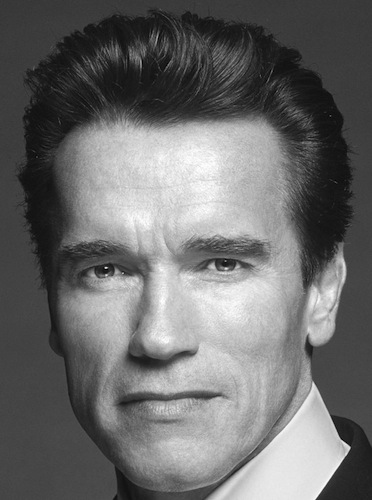
\includegraphics[height=1.5in]{../../rec/faces/arnold_schwarzenegger.jpg}
    }
    \subfigure[]{
        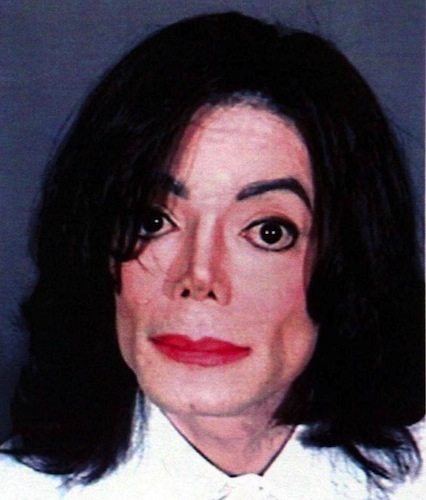
\includegraphics[height=1.5in]{../../rec/faces/michael_jackson.jpg}
    } \\
    \subfigure[]{
        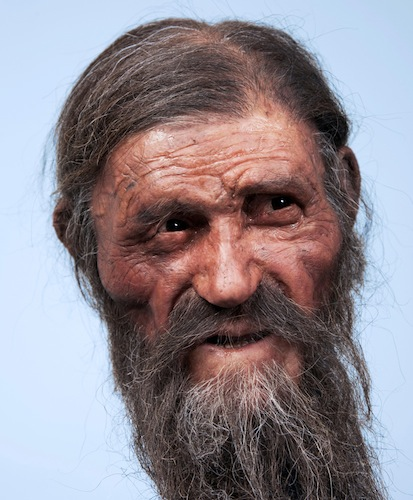
\includegraphics[height=1.5in]{../../rec/faces/old_man.jpg}
    }
    \subfigure[]{
        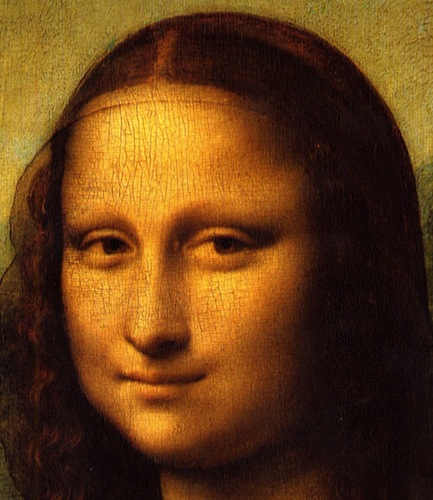
\includegraphics[height=1.5in]{../../rec/faces/mona_lisa.jpg}
    } \\
    \subfigure[]{
        \label{fig:faces:spongebob}
        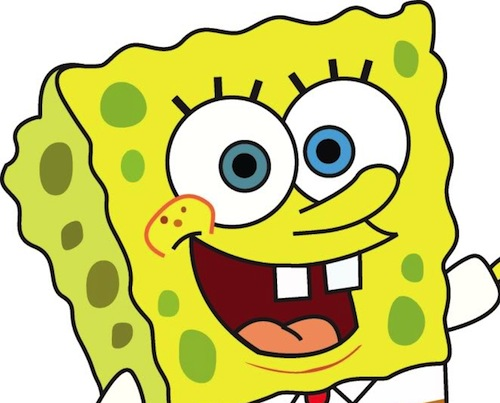
\includegraphics[height=1.5in]{../../rec/faces/spongebob.jpg}
    }
    \caption{Face images used in the experimentation.\label{fig:faces}}
\end{figure}

The diverse image set was chosen specifically to observe the effects of single distortions across a variety of faces. In many cases the same effect is achieved, in some cases some quite diverse effects are seen (especially when dealing with the oddly proportioned cartoon figure). Of course the same mathematical function is being performed, but the proportions of the face along with the structure have an impact on what human observers interpret to have happened to the face.

Generally for each image the interactive evolutionary process is conducted by the operators (independently). The different faces are evolved individually to determine what effects a distortion desirable on one image has on the rest of the set. Throughout the evolution there were a few tools at the disposal of the operator. The most intuitive operation is the operator selection of favored images followed by a single generation evolution step. This is a fairly slow but also quite tailored approach to the process.

In some instances the population might be highly homogeneous with only slight distortions between images. If this is not desirable, the cross correlation boost method can be used which will, over some user specified number of generations, select images from the population which are not highly correlated with others in the selection. For the correlation, the brightness map of each image is calculated and added one at a time to the selection. The images are only added if there is a large amount of dissimilarity between the two, which is determined with a two dimensional correlation with each image already in the selection. This does a reasonable job of adding some additional diversity in the set.

One pitfall of the cross-correlation approach is that it's quite slow, primarily because the output images have to be calculated for each generation. This process is sped up considerably as the evolutionary application uses scaled down versions of the original image, a process made possible by the use of a normalized image coordinate space, but the correlation and output calculation especially still take a noticeable amount of time to compute. The cross correlation method is useful to gain some diversity, but if a boost in complexity is desired the uncorrelated boost feature can be used which does not correlate any images, nor does it ever even calculate the output of the networks for all but the last set to be displayed to the operator. In this approach, members of the population are randomly assigned a fitness. The benefit here is that a large number of generations can be executed extremely which can be useful in order to gain complexity (or potentially to remove complexity, depending on how the evolutionary parameters are configured).

As alluded to, the operator is able to modify the NEAT parameters at any time to affect the evolutionary process. If more complexity is desired, for example, the node or link creation parameters may be increased. If less complexity is desired, the same parameters may be decreased along with the increase of the node and link destruction parameters. The experiments run for this project included a variety of the methods described above.

Once a favorable distortion has been evolved, the distortion is stored then applied across all images in the set for comparison.